\documentclass[12pt,twoside]{report}

% some definitions for the title page
\newcommand{\reporttitle}{Transfer Learning for Deep Learning Radiotherapy Planning}
\newcommand{\reportauthor}{Anton Zhitomirsky}
\newcommand{\supervisor}{Prof Ben Glocker}
\newcommand{\secondMarker}{Dr Thomas Heinis}
\newcommand{\reporttype}{MEng Individual Project}

% load some definitions and default packages
%%%%%%%%%%%%%%%%%%%%%%%%%%%%%%%%%%%%%%%%%
% University Assignment Title Page 
% LaTeX Template
% Version 1.0 (27/12/12)
%
% This template has been downloaded from:
% http://www.LaTeXTemplates.com
%
% Original author:
% WikiBooks (http://en.wikibooks.org/wiki/LaTeX/Title_Creation)
%
% License:
% CC BY-NC-SA 3.0 (http://creativecommons.org/licenses/by-nc-sa/3.0/)
% 
%
%%%%%%%%%%%%%%%%%%%%%%%%%%%%%%%%%%%%%%%%%
%----------------------------------------------------------------------------------------
%	PACKAGES AND OTHER DOCUMENT CONFIGURATIONS
%----------------------------------------------------------------------------------------
\usepackage[a4paper,hmargin=2.0cm,vmargin=1.0cm,includeheadfoot]{geometry}
\usepackage{textpos}

\usepackage[square,numbers]{natbib} % for bibliography
\usepackage[nottoc]{tocbibind} % Includes "References" in the table of contents
\bibliographystyle{unsrtnat}

\usepackage{tabularx,longtable,multirow,subfigure,caption}%hangcaption
\usepackage{fancyhdr} % page layout
\usepackage{url} % URLs
\usepackage[english]{babel}
\usepackage{amsmath}
\usepackage{graphicx}
\usepackage{scalerel}
\usepackage{dsfont}
\usepackage{epstopdf} % automatically replace .eps with .pdf in graphics
\usepackage{backref} % needed for citations
\usepackage{array}
\usepackage{latexsym}

\usepackage[pdftex,pagebackref,hypertexnames=false,colorlinks]{hyperref} % provide links in pdf
\usepackage{booktabs}
\usepackage{wrapfig}
\usepackage{caption}  % Required for \captionof
\usepackage{float} % for H option in figures
\usepackage{amssymb}
\usepackage{amsmath}
\usepackage{csquotes}
% \usepackage{subcaption} % causes a compilation error after changing back to natbib referencing... 

\hypersetup{pdftitle={},
  pdfsubject={}, 
  pdfauthor={},
  pdfkeywords={}, 
  pdfstartview=FitH,
  pdfpagemode={UseOutlines},% None, FullScreen, UseOutlines
  bookmarksnumbered=true, bookmarksopen=true, colorlinks,
    citecolor=black,%
    filecolor=black,%
    linkcolor=black,%
    urlcolor=black}

\usepackage[all]{hypcap}

%%%%%%%%%%%%%%%%%%%%%%%%%%%%%%%%%%%%%%%%%%%%%%%%%%%%%%%%%%%%%%%%%%%%%%%%%%%%%%%%
% LISTINGS ammendments
%%%%%%%%%%%%%%%%%%%%%%%%%%%%%%%%%%%%%%%%%%%%%%%%%%%%%%%%%%%%%%%%%%%%%%%%%%%%%%%%
\usepackage{listings}

\lstset
{ %Formatting for code in appendix
    language=Matlab,
    basicstyle=\footnotesize,
    % numbers=left,
    stepnumber=1,
    showstringspaces=false,
    tabsize=1,
    breaklines=true,
    breakatwhitespace=false,
    frame=single,
    columns=fullflexible,
    postbreak=\mbox{\textcolor{red}{$\hookrightarrow$}\space},
}

%\usepackage{color}
%\usepackage[tight,ugly]{units}
%\usepackage{float}
%\usepackage{tcolorbox}
%\usepackage[colorinlistoftodos]{todonotes}
% \usepackage{ntheorem}
% \theoremstyle{break}
% \newtheorem{lemma}{Lemma}
% \newtheorem{theorem}{Theorem}
% \newtheorem{remark}{Remark}
% \newtheorem{definition}{Definition}
% \newtheorem{proof}{Proof}


%%% Default fonts
\renewcommand*{\rmdefault}{bch}
\renewcommand*{\ttdefault}{cmtt}


%%% Default settings (page layout)
\setlength{\parindent}{0em}  % indentation of paragraph
\setlength{\parskip}{.3em}

% \setlength{\parindent}{0em}  % indentation of paragraph

\setlength{\headheight}{14.5pt}
\pagestyle{fancy}
\renewcommand{\chaptermark}[1]{\markboth{\chaptername\ \thechapter.\ #1}{}}
%\fancyhead[RO]{\sffamily \textbf{\thepage}} %Page no.in the right on even pages
%\fancyhead[LE]{\sffamily \textbf{\thepage}} %Page no. in the left on odd pages

\fancyfoot[ER,OL]{\thepage}%Page no. in the left on
%odd pages and on right on even pages
\fancyfoot[OC,EC]{\sffamily }
\renewcommand{\headrulewidth}{0.1pt}
\renewcommand{\footrulewidth}{0.1pt}
\captionsetup{margin=10pt,font=small,labelfont=bf}


%--- chapter heading

\def\@makechapterhead#1{%
  \vspace*{10\p@}%
  {\parindent \z@ \raggedright \sffamily
    \interlinepenalty\@M
    \Huge\bfseries \thechapter \space\space #1\par\nobreak
    \vskip 30\p@
  }}

%--- chapter heading

\def\@makechapterhead#1{%
  \vspace*{10\p@}%
  {\parindent \z@ \raggedright \sffamily
    %{\Large \MakeUppercase{\@chapapp} \space \thechapter}
    %\\
    %\hrulefill
    %\par\nobreak
    %\vskip 10\p@
    \interlinepenalty\@M
    \Huge\bfseries \thechapter \space\space #1\par\nobreak
    \vskip 30\p@
  }}

%---chapter heading for \chapter*  
\def\@makeschapterhead#1{%
  \vspace*{10\p@}%
  {\parindent \z@ \raggedright
    \sffamily
    \interlinepenalty\@M
    \Huge \bfseries  #1\par\nobreak
    \vskip 30\p@
  }}
\allowdisplaybreaks

% load some macros
% Here, you can define your own macros. Some examples are given below.

\newcommand{\R}[0]{\mathds{R}} % real numbers
\newcommand{\Z}[0]{\mathds{Z}} % integers
\newcommand{\N}[0]{\mathds{N}} % natural numbers
\newcommand{\C}[0]{\mathds{C}} % complex numbers
% \renewcommand{\vec}[1]{{\boldsymbol{{#1}}}} % vector
\newcommand{\mat}[1]{{\boldsymbol{{#1}}}} % matrix

\usepackage{pifont,mdframed}
\newenvironment{warning}
  {\par\begin{mdframed}[linewidth=1pt,linecolor=black]%
    \begin{list}{}{\leftmargin=1cm
                  \labelwidth=\leftmargin}\item[\Large\ding{43}]}
  {\end{list}\end{mdframed}\par}

\definecolor{lightgray}{gray}{0.9}

% load title page
\begin{document}
% Last modification: 2015-08-17 (Marc Deisenroth)
\begin{titlepage}

    \newcommand{\HRule}{\rule{\linewidth}{0.5mm}} % Defines a new command for the horizontal lines, change thickness here
    
    %----------------------------------------------------------------------------------------
    %	LOGO SECTION
    %----------------------------------------------------------------------------------------
    
    
\includegraphics[width = 4cm]{../figures/imperial.pdf}\\[0.5cm] 
    
    \center % Center everything on the page
     
    %----------------------------------------------------------------------------------------
    %	HEADING SECTIONS
    %----------------------------------------------------------------------------------------
    
    \textsc{\LARGE \reporttype}\\[1.5cm] 
    \textsc{\Large Department of Computing}\\[0.5cm] 
    \textsc{\large Imperial College of Science, Technology and Medicine}\\[0.5cm] 
    
    %----------------------------------------------------------------------------------------
    %	TITLE SECTION
    %----------------------------------------------------------------------------------------
    
    \HRule \\[0.4cm]
    { \huge \bfseries \reporttitle}\\ % Title of your document
    \HRule \\[1.5cm]
     
    %----------------------------------------------------------------------------------------
    %	AUTHOR SECTION
    %----------------------------------------------------------------------------------------
    
    \begin{minipage}{0.4\textwidth}
    \begin{flushleft} \large
    \emph{Author:}\\
    \reportauthor % Your name
    \end{flushleft}
    \end{minipage}
    ~
    \begin{minipage}{0.4\textwidth}
    \begin{flushright} \large
    \emph{Supervisor:} \\
    \supervisor % Supervisor's Name
    \end{flushright}
    \end{minipage}\\[4cm]
    
    
    
    
    %----------------------------------------------------------------------------------------
    
    
    %----------------------------------------------------------------------------------------
    %	DATE SECTION
    %----------------------------------------------------------------------------------------
    
    {\large \today} % Date, change the \today to a set date if you want to be precise
    
    
    \vfill % Fill the rest of the page with whitespace
    Submitted in partial fulfillment of the requirements for the \degreetype~of Imperial College London
    
    \end{titlepage}
    

% page numbering etc.
\pagenumbering{roman}
\clearpage{\pagestyle{empty}\cleardoublepage}
\setcounter{page}{1}
\pagestyle{fancy}

% \cleardoublepage
%%%%%%%%%%%%%%%%%%%%%%%%%%%%%%%%%%%%
% \section*{Acknowledgments}
% Comment this out if not needed.

% \clearpage{\pagestyle{empty}\cleardoublepage}

%%%%%%%%%%%%%%%%%%%%%%%%%%%%%%%%%%%%

% \begin{abstract}\label{sect:abstract}
   
% \end{abstract}
  
%%%%%%%%%%%%%%%%%%%%%%%%%%%%%%%%%%%%
%--- table of contents
\fancyhead[RE,LO]{\sffamily {Table of Contents}}
\tableofcontents
  
% \clearpage{\pagestyle{empty}\cleardoublepage}

%%%%%%%%%%%%%%%%%%%%%%%%%%%%%%%%%%%%

\pagenumbering{arabic}
\setcounter{page}{1}
\fancyhead[LE,RO]{\slshape \rightmark}
\fancyhead[LO,RE]{\slshape \leftmark}

%%%%%%%%%%%%%%%%%%%%%%%%%%%%%%%%%%%%
\chapter{Introduction}



\section{Technical Context}

% To mention: Medical Image Segmentation is currently dominated by deep convolutional neural networks (CNNs). However, each segmentation benchmark seems to require specialized architectures and training scheme modifications to achieve competi- tive performance [1,2,3,4,5]. This results in huge amounts of publications in the field that, alongside often limited validation on only few or even just a single dataset, make it increasingly difficult for researchers to identify methods that live up to their promised superiority beyond the limited scenarios they are demon- strated on~\cite{nnunet}

% In many biomedical applications, only very few images are required to train a network that generalizes reasonably well. This is because each image already comprises repetitive structures with corresponding variation~\cite{DBLP:journals/corr/CicekALBR16}.

\section{Objectives and Contributions}

\section{Outline of Report}

The report will first discuss the relevant background knowledge required for this project in Chapter~\ref{sect:motivation}. Within, we provide a high-level overview of anatomies and the clinical context (Section~\ref{sect:clinical-context}) as well as core existing academic knowledge in the Computer-assisted vision in the Medical Imaging field (Section~\ref{sect:machine-learning-for-image-segmentation}-\ref{sect:performance-evaluation}). 

Then, Chapter~\ref{sect:methodology} describes the experiments used to evaluate how well different architectures transfer knowledge into the target domain, as well as an overview of the results (Chapter~\ref{sect:results}) as well as a discussion of their implications (Chapter~\ref{sect:discussion}).

%%%%%%%%%%%%%%%%%%%%%%%%%%%%%%%%%%%%
\chapter{Motivation}\label{sect:motivation}

\section{Clinical Context}\label{sect:clinical-context}

This project will have its foundation for experimentation in a dataset provided by the Royal Marsden Hospital. The real-world clinical dataset segments key anatomies and tumours that aid in radiotherapy planning for females with cervical cancer. It has yet to gain exposure to the widespread segmentation challenges and has uncommon and limited segmentation patterns. This dataset will act as the pillar for justifying the success of the transferability of knowledge between medical domains.

In this section, we discuss the clinical context behind cervical cancer in the population, the Hospital's pipeline for segmenting patients in preparation for radiotherapy treatment, and the Hospital's motivation for recruiting an AI tool to assist in its treatment pipeline. 

\subsection{Cervical Cancer}\label{sect:cervical-cancer}

Cancer is a burden around the globe that has been a driver for almost one-sixth of the world's mortality in 2022~\cite{Global-cancer-2022}. In females, cervical cancer makes up 25 countries' leading causes of cancer death, following breast cancer for 157 countries in 2022~\cite{Global-cancer-2022}. Furthermore, an estimated 1 million maternal orphans who lose their mothers to cancer suffer long-term disadvantages in health and education~\cite{Guida2022}. Thankfully, cancer screening services provided by hospitals around Europe have been shown to decrease incidence and mortality rates of cervical cancer in women over the recent years~\cite{Global-cancer-2022}, which inspires further complete clinical understanding of the disease. Paired with quality improvements offered by medical imaging models, the motivation for total control over cervical cancer drive this research project to explore transfer knowledge in this field. % TODO: have you mentioned that transfer learning is a gap in the field?

\subsection{Radiotherapy Treatment}

A mechanism available for cancer treatment involves radiation therapy. High beams of radiation energy are tuned to hone in to target cancerous cells in a clinically defined 'target area'. The cells killed by the energy experience interphase or proliferative death depending on the cell cycle stage. Death occurs when the damage to genetic material within the cell prevents it from dividing, or the cell's accumulation of genetic aberrations leads to a ``mitotic catastrophe''~\cite{cell-death}. In Europe, radiotherapy treatment was used on average for 70\% of cases, with a curative rate of 40\%~\cite{radiotherapy-advances, Thompson2018}.

This death is characteristic of any cell subjected to high energy beams, placing much responsibility on the Oncologist to deliver an accurate treatment area so that healthy cells are unaffected; any adverse alteration of an organ's standard functionality may cause grave implications for the already compromised patient. Therefore, the precise and complex nature of the task is estimated to take oncologists 90-120 mins to delineate target areas for radiotherapy~\cite{LIU2020184}.

This time-consuming endeavour is never favourable for a patient already in a dangerous situation. For mid-low-income countries, where this may not be an available resource, this leaves them with a death rate 18 times that of a higher-income country~\cite{cervical-cancer-epidemic}. 

\subsection{CT modality}

High-resolution and high-contrast CT machines have further benefited cancer treatment due to their noninvasive nature and ability to view patients' internal organs. X-ray devices rotate around a specified body part, and computer-generated cross-sectional images are produced~\cite{file-formats}. Whilst the scanner rotates, the patient's table slowly moves up and down inside the tube to produce different cross-section images. The images show damaged and surrounding soft tissue, allowing physicians to propose clinical target volumes more accurately.

\subsubsection{Hounsfield Units}

\begin{figure}[H]
    \centering
    \subfigure[Muscle Window $(35,55)$~\cite{other-HD-units}]{{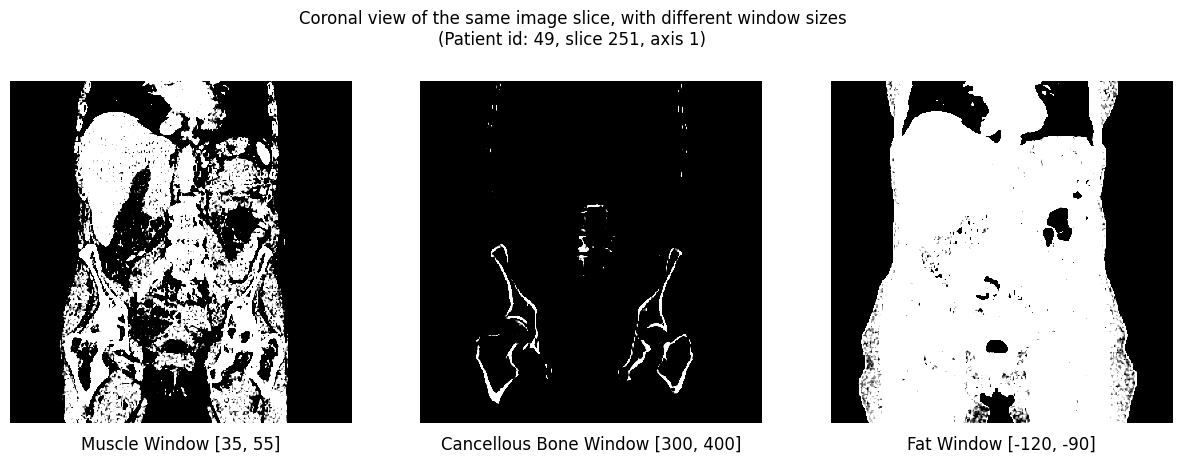
\includegraphics[width=0.3\textwidth, trim=0.2cm 1cm 21cm 2cm, clip]{../figures/HU-window.png}}}
    \subfigure[Cancellous Bone Window  $(300,400)$~\cite{cancellous-bone}]{{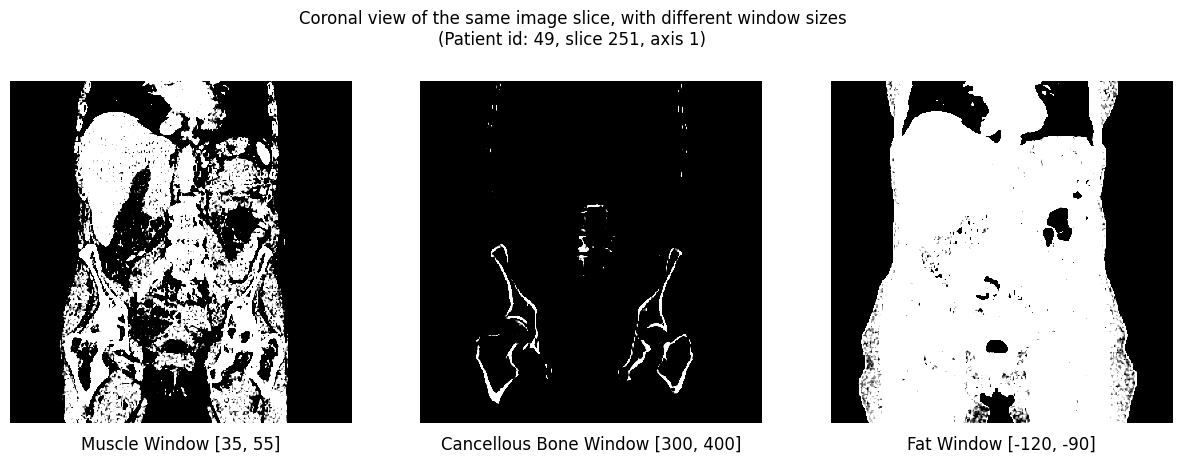
\includegraphics[width=0.3\textwidth, trim=10.6cm 1cm 10.6cm 2cm, clip]{../figures/HU-window.png}}}
    \subfigure[Fat Window $(-120, -90)$~\cite{other-HD-units}]{{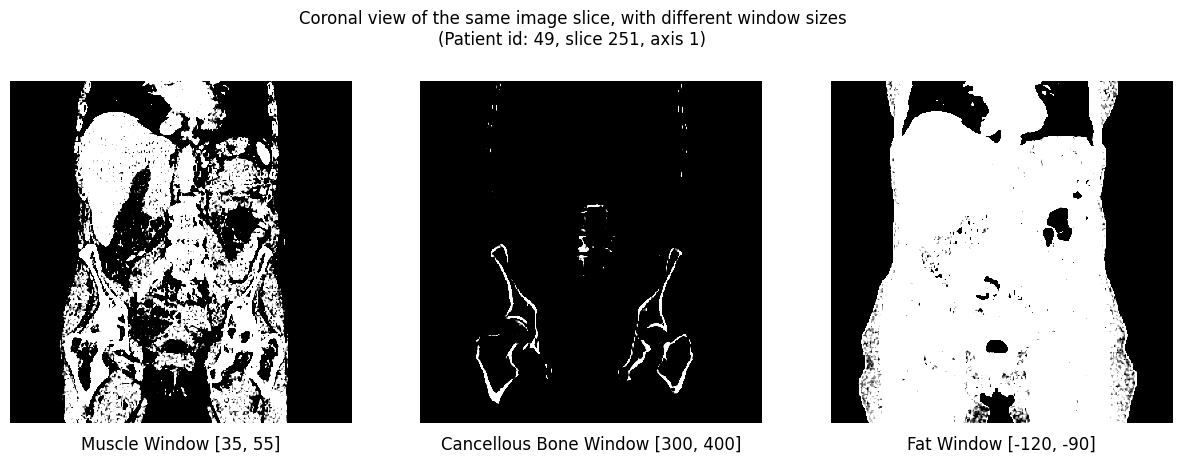
\includegraphics[width=0.3\textwidth, trim=21cm 1cm 0.2cm 2cm, clip]{../figures/HU-window.png}}}
    \caption{Coronal view the same image slice of a CT image, with different window cropping (Patient id: 49, slice 251). White areas represent high-density tissues, and black areas represent low-density tissues within the window range.}
    \label{fig:ct-windows}
\end{figure}

The operator or physician decides the granularity or image slice thickness, which ranges from 1mm to 10mm. Therefore, the precision along each axis creates a cube, or voxel, representing the value on a grid in three-dimensional space. The voxel values are measured in Hounsfield Units (HU)~\cite{diagnostic-radiology-physics}. 

Contrary to natural images, where pixel values vary from 0 to 255 in 3 channels representing Red, Blue and Green, the Hounsfield scale is a quantitative scale describing radiodensity. The image intensity reflects tissue type; each voxel intensity refers to a specific tissue composition. The positive values (white) result from more dense tissue with greater X-ray beam absorption, and negative values (black) are less dense tissue with less X-ray beam absorption~\cite{Statpearls}.  

Therefore, because the HU scale is relative, different windows may be taken for a CT scan to highlight different tissues. Those voxels within the window will likely be tissues of a specific classification. For example, as shown in Figure~\ref{fig:ct-windows}, we display three such windows: muscle, cancellous bone and fat.

\subsection{Radiotherapy Planning}\label{sect:radiotherapy-planning}

\begin{warning}
  Perhaps, include a graph to visualse target volumes visually
\end{warning}

Oncologist use the CT scans to draw clinical volumes by combining their knowledge about the particular cancer to determine target structures, organs-at-risk structures, and areas where the cancer will likely spread to~\cite{AMLART-data}. 

The first area is the macroscopic delineated area of the visible tumour area. This Gross Target Volume (GTV) has a high probability of containing the tumour. Secondly, the Clinical Target Volume (CTV) is derived to account for potential microscopic spread. The CTV will be an area at least as big as the GTV with an optional margin surrounding it containing a 'rind' of non-zero probability of tumour spread. Lastly, the Primary Target Volume (PTV) contains residual geometric uncertainties and safety margins surrounding the CTV, ensuring the radiotherapy dose gets delivered to the CTV~\cite{tumor-delineation,defining-target-volumes,Lin2021-oz,personalised-PTV-strategies}. The PTV is a necessary extension of the CTV since geometric uncertainties are impossible and not advised to eliminate; after all, static scans are only estimations, subject to short-term organ misalignment, relative movement between structures of reference and tumours, partial volume effects and skewed anisotropic resolution~\cite{VANHERK200452}.

In parallel, the Oncologist constantly considers critical healthy tissue structures that need to be preserved during irradiation. These are referred to as organs-at-risk (ORs). In some specific circumstances, adding a margin analogous to the PTV margin around an OR is necessary to ensure that the organ cannot receive a higher-than-safe dose; this gives a planning organ at risk volume~\cite{defining-target-volumes}.

\subsection{International Guidelines}

The final volumes have no internationally agreed-upon guidelines, which leaves it up to the interpretation of the oncologists and Hospitals to use their heuristics when drawing areas. This time-consuming process has high variability, causing it to suffer significantly from inter and intra-observer variability~\cite{Lin2021-oz}. 

% However, the data provided has been standardised as a gold standard; see Section~\ref{sect:data}.

\subsection{Data Aquisition}

The Royal Marsden Hospital provides the dataset as a set of `Neuroimaging Informatics Technology Initiative' files (NIfTI)~\cite{file-formats}. It is a lightweight alternative to other formats such as DICOM and eliminates ambiguity from spatial orientation information~\cite{dicom-to-nifti-conversion}. Libraries exist for handling these files, such as SimpleITK~\cite{SimpleITK-paper}, which we use to read and manipulate the data in this project. % The library reads, manipulates, and handles the image as a set of points in a grid occupying a physical region in space defined by the metadata to remove ambiguity from the origin, size, spacing, and so on that might vary between patient scans.

The training data provides one hundred female patients that have been diagnosed with similar types of cervical cancer. Each patient comes with seven relevant segmentation classes which contribute to radiotherapy planning for cervical cancer. For reproducibility, all delineated anatomies were labelled consistently by the Oncologists to improve chances that an AI model can learn cervical cancer patterns~\cite{AMLART-data}. 

Finally, the dataset comes with ten hold-out data items, which are patients with only the raw CT scan information without labels.

% \subsubsection{Notes}

% Some notes contain clinical observations about each of the 100 labelled data pairs~\cite{AMLART-data}. This small sample size of patients is also a good representation of the variability of data in the population. Because of the relatively small sample size, it is essential to be more acutely aware of the variability in the data.

% A common observation is that scans contain poor contrast. For patient 13, the note reads ``no contrast - hard to see LNs,'' which is information crucial to determining segmenting the Clinical Target Volume for Lymph Nodes (CTVn). Patients 9, 60, and 62 also have ``very large tumours''; sometimes, these even shift into uncommon areas, with ``sigmoid hanging into parametrium''. % GTV not visible?

% The notes help identify and diagnose some reasons for the model's poor performance in some cases, which may be due to the high variability between patients in quality and physiology.

\subsection{Delineation classes}



The clinicians at the Royal Marsden Hospital have provided segmentation labels for seven high-priority regions of interest (roi). These are the Bladder, Anorectum, CTVn, CTVp, Parametrium, Uterus, and Vagina. The function of these anatomies is irrelevant to this project and is left to the reader to research further.

\subsubsection{Organs At Risk}\label{sec:data-organs-at-risk}

\begin{figure}[H]
  \centering
  \subfigure[Axial]{
    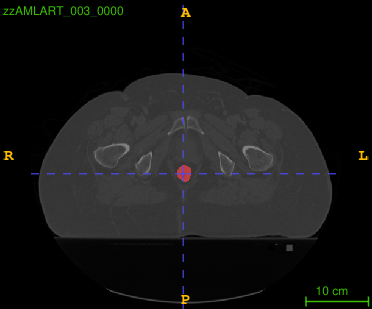
\includegraphics[width=0.3\textwidth]{../figures/PatientStructureExamples/Anorectum_003/Axial.png}
   \label{fig:example-anorectum-axial}
  }
  \subfigure[Coronal]{
    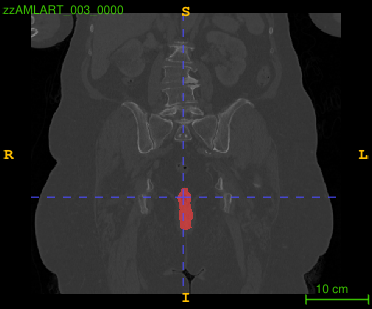
\includegraphics[width=0.3\textwidth]{../figures/PatientStructureExamples/Anorectum_003/Coronal.png}
   \label{fig:example-anorectum-coronal}
  }
  \subfigure[Sagittal]{
    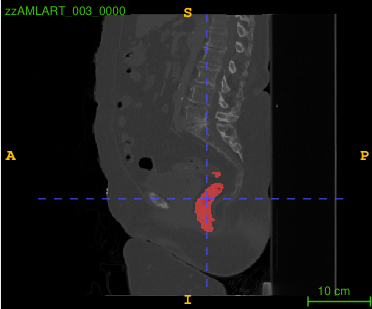
\includegraphics[width=0.3\textwidth]{../figures/PatientStructureExamples/Anorectum_003/Sagittal.png}
   \label{fig:example-anorectum-sagittal}
  }
  \subfigure[Axial]{
    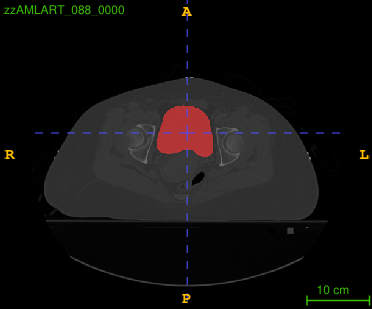
\includegraphics[width=0.3\textwidth]{../figures/PatientStructureExamples/Bladder_088/Axial.png}
   \label{fig:example-bladder-axial}
  }
  \subfigure[Coronal]{
    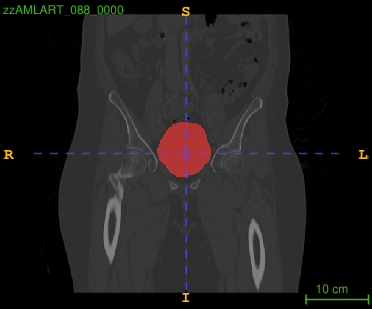
\includegraphics[width=0.3\textwidth]{../figures/PatientStructureExamples/Bladder_088/Coronal.png}
   \label{fig:example-bladder-coronal}
  }
  \subfigure[Sagittal]{
    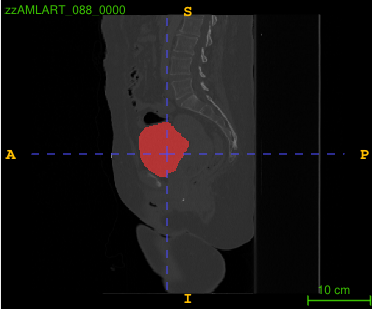
\includegraphics[width=0.3\textwidth]{../figures/PatientStructureExamples/Bladder_088/Sagittal.png}
   \label{fig:example-bladder-sagittal}
  }
  \caption{Views of the segmentation (in red) of the Anorectum (\ref{fig:example-anorectum-axial}-\ref{fig:example-anorectum-sagittal}) and  the segmentation (in red) of the Bladder (\ref{fig:example-bladder-axial}-\ref{fig:example-bladder-sagittal}) of an arbitrary patient}
\end{figure}

An organ at risk is an organ that, despite being healthy, is substantially likely to be within the PTV. Any areas created around the area should actively avoid these organs because overlapping with them risks complicating treatment and compromising the health of functioning organs. The key supplied anatomies at risk are the  Anorectum (Figure~\ref{fig:example-anorectum-axial}-\ref{fig:example-anorectum-sagittal}) and the Bladder (Figure~\ref{fig:example-bladder-axial}-\ref{fig:example-bladder-sagittal}).

\subsubsection{CTVp}\label{sec:data-CTVp}

\begin{figure}[H]
  \centering
  \subfigure[Axial]{
    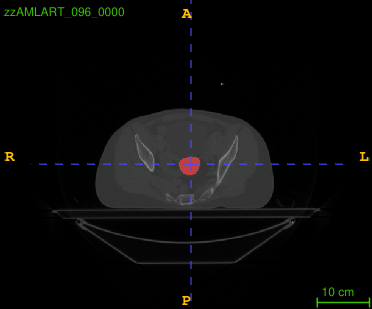
\includegraphics[width=0.3\textwidth]{../figures/PatientStructureExamples/CTVp_096/Axial.png}
   \label{fig:example-CTVp-axial}
  }
  \subfigure[Coronal]{
    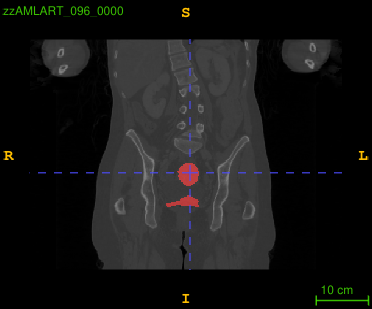
\includegraphics[width=0.3\textwidth]{../figures/PatientStructureExamples/CTVp_096/Coronal.png}
   \label{fig:example-CTVp-coronal}
  }
  \subfigure[Sagittal]{
    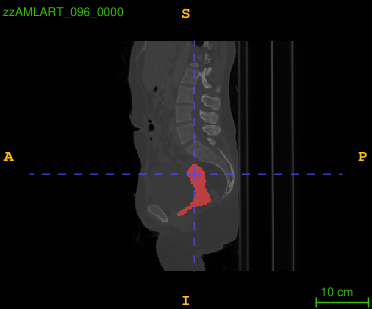
\includegraphics[width=0.3\textwidth]{../figures/PatientStructureExamples/CTVp_096/Sagittal.png}
   \label{fig:example-CTVp-sagittal}
  }
  \caption{Views of a segmented (in red) CTVp of an arbitrary patient}
 \label{fig:example-CTVp}
\end{figure}

The CTVp stands for the Primary Clinical Target Volume; see the example at Figure~\ref{fig:example-CTVp}. This is an area comprised from areas where there may be local microscopic spread (uterus, cervix, upper vagina, primary tumour)~\cite{AMLART-data}.

\subsubsection{CTVn}\label{sec:data-CTVn}

\begin{figure}[H]
  \centering
  \subfigure[Axial]{
    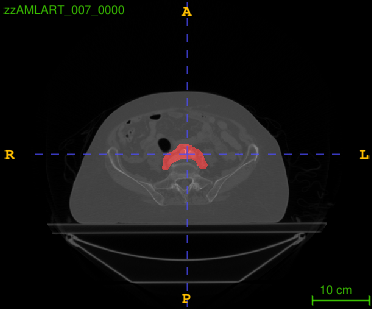
\includegraphics[width=0.3\textwidth]{../figures/PatientStructureExamples/CTVn_007/Axial.png}
   \label{fig:example-CTVn-axial}
  }
  \subfigure[Coronal]{
    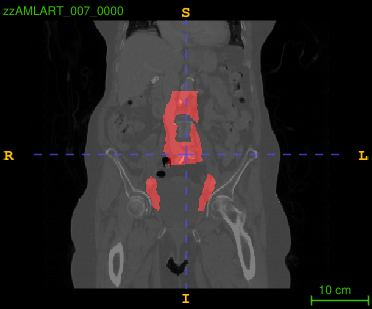
\includegraphics[width=0.3\textwidth]{../figures/PatientStructureExamples/CTVn_007/Coronal.png}
   \label{fig:example-CTVn-coronal}
  }
  \subfigure[Sagittal]{
    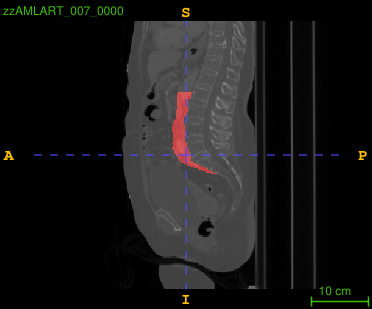
\includegraphics[width=0.3\textwidth]{../figures/PatientStructureExamples/CTVn_007/Sagittal.png}
   \label{fig:example-CTVn-sagittal}
  }
  \caption{Views of a segmented (in red) CTVn of an arbitrary patient}
 \label{fig:example-CTVn}
\end{figure}

The CTVn stands for Nodal Clinical Target Volume; see the example at Figure~\ref{fig:example-CTVn}. This CTV surrounds areas that may contain microscopic spread to lymph nodes. It is drawn based on set margins around pelvic blood vessels and includes pelvic lymph nodes, common iliac lymph nodes and para-aortic lymph nodes~\cite{AMLART-data}.

Similarly to CTVp, this is a compound area with three groups of lymph nodes. In clinical practice, the number of these groups in the CTV varies in each patient, depending on the advanced disease. % TODO: reference notes? They say that depending on the development of the disease, different patients may get different extents of contouring of this structure.
However, in contrast to the CTVp, this area is drawn depending on the development of the disease.

\subsubsection{Parametrium}\label{sec:data-Parametrium}

\begin{figure}[H]
  \subfigure[Axial]{
    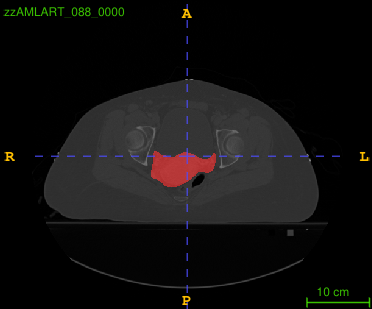
\includegraphics[width=0.3\textwidth]{../figures/PatientStructureExamples/Parametrium_088/Axial.png}
   \label{fig:example-Parametrium-axial}
  }
  \subfigure[Coronal]{
    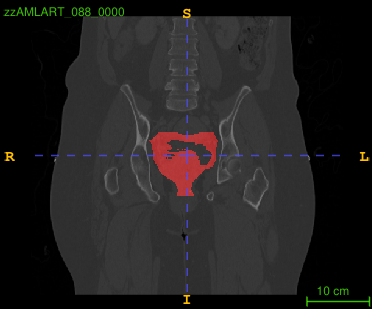
\includegraphics[width=0.3\textwidth]{../figures/PatientStructureExamples/Parametrium_088/Coronal.png}
   \label{fig:example-Parametrium-coronal}
  }
  \subfigure[Sagittal]{
    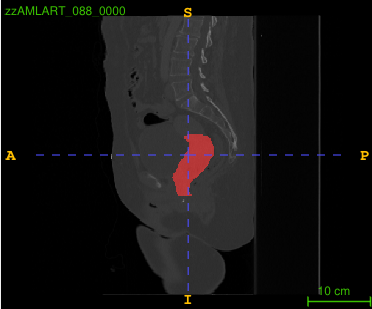
\includegraphics[width=0.3\textwidth]{../figures/PatientStructureExamples/Parametrium_088/Sagittal.png}
   \label{fig:example-Parametrium-saggital}
  }
  \caption{Views of a segmented (in red) Parametrium of an arbitrary patient}
 \label{fig:example-Parametrium}
\end{figure}

The Parametrium (or Paravagina) is the tissue surrounding the cervix/vagina - at risk of local spread; see Figure~\ref{fig:example-Parametrium}. The Parametrium is drawn as a complete structure and edited back to the level of the vagina to be included~\cite{AMLART-data}.

\subsubsection{Vagina and Uterus}

\begin{figure}[H]
  \centering
  \subfigure[Axial]{
    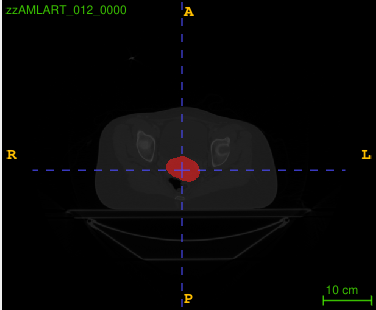
\includegraphics[width=0.3\textwidth]{../figures/PatientStructureExamples/Uterus_012/Axial.png}
   \label{fig:example-uterus-axial}
  }
  \subfigure[Coronal]{
    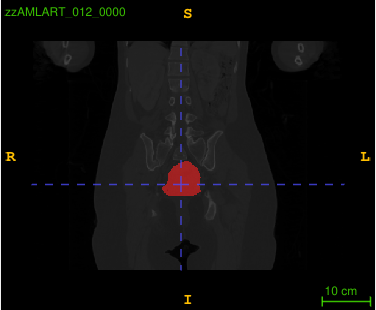
\includegraphics[width=0.3\textwidth]{../figures/PatientStructureExamples/Uterus_012/Coronal.png}
   \label{fig:example-uterus-coronal}
  }
  \subfigure[Sagittal]{
    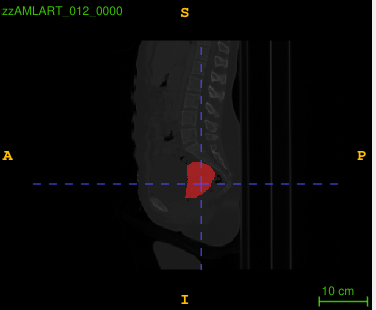
\includegraphics[width=0.3\textwidth]{../figures/PatientStructureExamples/Uterus_012/Sagittal.png}
   \label{fig:example-uterus-sagittal}
  }
  \subfigure[Axial]{
    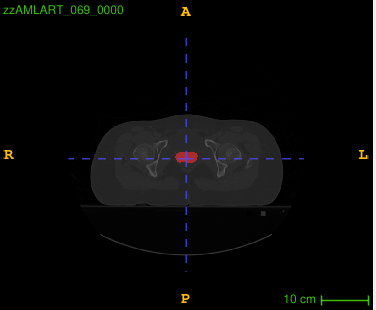
\includegraphics[width=0.3\textwidth]{../figures/PatientStructureExamples/Vagina_69/Axial.png}
   \label{fig:example-vagina-axial}
  }
  \subfigure[Coronal]{
    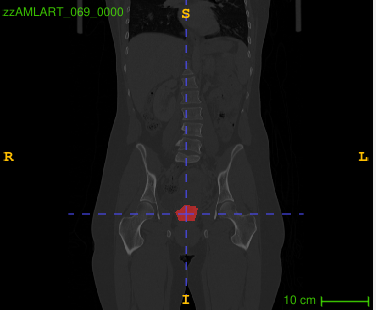
\includegraphics[width=0.3\textwidth]{../figures/PatientStructureExamples/Vagina_69/Coronal.png}
   \label{fig:example-vagina-coronal}
  }
  \subfigure[Sagittal]{
    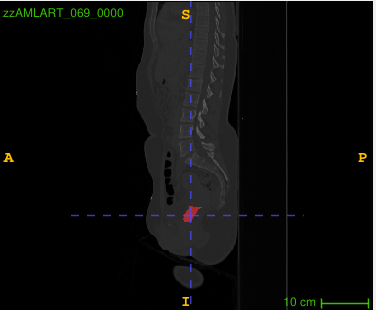
\includegraphics[width=0.3\textwidth]{../figures/PatientStructureExamples/Vagina_69/Sagittal.png}
   \label{fig:example-vagina-sagittal}
  }
  \caption{Views of the segmentation (in red) of the Uterus (\ref{fig:example-uterus-axial}-\ref{fig:example-uterus-sagittal}) and  the segmentation (in red) of the Vagina (\ref{fig:example-vagina-axial}-\ref{fig:example-vagina-sagittal}) of an arbitrary patient}
\end{figure}
The final structures are the Vagina and Uterus, their clinical significance is to help define encapsulating structures like the CTVn (see Section~\ref{sec:data-delineation-rules}).

\subsection{Rules}\label{sec:data-delineation-rules}

Let us represent each organ anatomy as the first letter of its name, specifically: ($A$)norectum, ($B$)ladder, ($C$)ervix, ($P$)arametrium, ($U$)terus, ($V$)agina. Further, define:

\begin{enumerate}
  \item The CTVn and CTVp as $C_n$ and $C_p$ respectively
  \item The GTVn and GTVp as $G_n$ and $G_p$ respectively
  \item The Pelvic, Common and Para-aortic Lymph Node as $L_p$, $L_c$, and $L_{pa}$ respectively
\end{enumerate}

% \begin{minipage}{0.5\textwidth}
%   \subsubsection{Notation of Structures}
%   \begin{enumerate}
%     \item Let the Anorectum be denoted as $A$
%     \item Let the Bladder be denoted as $B$
%     \item Let the Cervix be denoted with $C$
%     \item Let the CTVn be denoted with $C_n$
%     \item Let the CTVp be denoted with $C_p$
%     \item Let the GTVp be denoted with $G_p$
%     \item Let the GTVn be denoted with $G_n$
%   \end{enumerate}
% \end{minipage}%
% \begin{minipage}{0.5\textwidth}

%   \begin{enumerate}
%     \setcounter{enumi}{7}
%     \item Let the Pelvic Lymph Node be denoted as $L_p$
%     \item Let the Common Iliac Lymph Node be denoted as $L_i$
%     \item Let the Para-aortic Lymph Node be denoted as $L_{pa}$
%     \item Let the Parametrium be denoted with $P$
%     \item Let the Uterus be denoted with $U$
%     \item Let the Vagina be denoted with $V$
%   \end{enumerate}

% \end{minipage}

\subsubsection{Relationship between Structures}

  \begin{enumerate}
    \item If we want to talk about a specific patient, we should use the super-script notation to differentiate patients, e.g., $B^i$ for the Bladder of patient $i$.
    \item Let the overlap of two structures be denoted by the set intersect symbol $\cap$.
    \item Let the joint area of two structures be denoted by the set union symbol $\cup$.
  \end{enumerate}

  % \vspace{4em}

The top seven priority structures have been selected to identify and plan an area where radiotherapy should be used. With these structures, there are rules that the clinicians have outlined, they are quoted for clarification (these structures only refer to each independent patient):

\begin{enumerate}
  \item There should be no overlap between the CTVn, CTVp or Anorectum.

        \begin{equation}
          \forall{i,j \in \{C_n, C_p, A\}}\text{ with } i \neq j, i \cap j = \emptyset
        \end{equation}

  \item The Parametrium may overlap with all of the other structures.

        \begin{equation}
          \forall i \in S, \quad P \cap S_i \neq \emptyset \vee P \cap S_i = \emptyset
        \end{equation}

  \item The Bladder may overlap with the CTVn.

        \begin{equation}
          B \cap C_n \neq \emptyset \vee B \cap C_n = \emptyset\label{eq:ctvn}
        \end{equation}

  \item The CTVp is defined as a compound structure containing:

        \begin{equation}
          C_p = \overbrace{C \cup G_p}^{\text{High Risk CTV}} \cup \ \ U \cup V\label{eq:ctvp1}
        \end{equation}

  However, since we are never explicitly provided with the segmentation maps for the Cervix $C$ and the GTVp $G_p$, we cannot use as strong of a definition as above. Instead, we operate on the assumption that the union of the Uterus and Vagina is at least as big as the CTVp.

        \begin{equation}
          U \cup V \subseteq C_p\label{eq:ctvp2}
        \end{equation}

  \item The CTVn is defined as a compound structure containing:

        \begin{equation}
          C_n = G_n \cup L_i \cup L_p + L_{pa}
        \end{equation}

  Similarly, we are not provided segmentations for these areas, therefore, operating under no clinical knoweldge apart from the provided, cannot make any claims as to the composition of the CTVn.

\end{enumerate}

\subsection{Motivation in AI}

The medical sector has been a hotbed for AI research since researchers realised they could apply Convolutional Neural Networks (Section~\ref{sect:image-segmentation}) to medical image data. A branch of research dedicated itself to segmentation, which involves labelling individual pixels in the image according to which object or class they belong to. In dense classification, a model assigns every pixel to a specific class. Relevant to the direction of this project is determining the precise location and extent of organs or certain types of tissue, like ORs, CTV volumes, or other anatomies. 

The key objective of models trained for delineating target structures for this project is to see if an AI model can learn cervical cancer CTV pattern detection. The decision is complex as clinicians use information beyond the CT-imaging modality, such as how far along the tumour has progressed, and other clinical intuition to make proper judgements about the CTV volumes. Therefore, with this information missing from AI models, it is likely to misjudge target volumes, and a clinician will have to select which components of the CTV are required. However, a clinician will likely benefit from the time saved and improved consistency with the planning process if a trained model can produce the substructures required within the CTV that a clinician can review~\cite{AMLART-data}.

\section{Machine learning for image segmentation}\label{sect:machine-learning-for-image-segmentation}

Before popularising machine learning algorithms, strict and convoluted rule sets defined algorithms. These heuristically defined algorithms struggled to scale to complex problems and were often complicated or confusing to maintain. The typical task, however, does not warp easily into human intuition.

Algorithms began to emerge that fell into the classification of neural network models. Observations were rephrased and morphed into vectorised inputs, where each constituent of the vector represented a particular feature of the observation. For instance, the California Housing dataset~\cite{kelleypace1997} contains an input of 9 features (longitude, latitude, number of bathrooms, ...) and one target feature (house price). After pre-processing and strategising, this input would be vectorised and fed into a network with several layers. Within each layer, sets of tunable parameters would optionally change the number of features and learn a relationship between parameters using weights until the $1 \times 9$ vector finally translates into a scalar value indicating the house price. After many repetitions of learning from examples, the model would learn an approximation to the solution. These models were termed Multi-Layered Perceptrons (MLPs).

\subsection{Image Segmentation}\label{sect:image-segmentation}

The current machine learning approach didn't work well with image data. Up until that point, rich structures such as images were neglected, and matrices of gray-scale images were mutilated into flat vectors. This approach was necessary to feed the flattened image representation through the MLP. The issue with vectorising an image is that it loses its spatial context-driven awareness. 

At the same time, J. Hull, sponsored by the United States Postal Service, published a Database for Handwritten Text Recognition with the incentive of providing an extensive dataset of images of characters of variable writing mediums, isolation, overlap, and neatness to aid research efforts in developing accurate digit classification algorithms~\cite{JJHull1994}. Yann LeCunn et al.~\cite{Lenet1998} used this database to propose the first Convolutional Neural Network (CNN) for image processing, which preserved the input in its 2D glory by applying convolutions.

\begin{figure}[H]
  \centering
  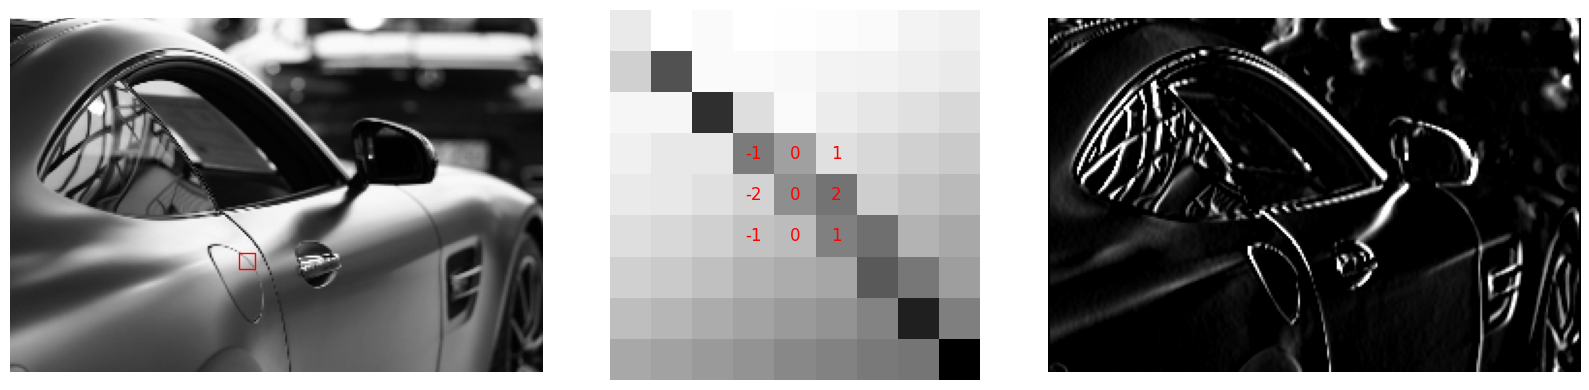
\includegraphics[width=1\linewidth]{../figures/sobel.png}
  \caption{Example application of a convolution. From left to right, the input image with a region outlined in a red box, the boxed region magnified with a convolutional (sobel) filter being applied to a part of the magnified region, and lastly the output after the filter has passed over the entire image. The output represents a new feature map encoding features of the original (input) feature.}\label{fig:sobel}
\end{figure}

Convolutional layers are rectangular blocks that are recipes for translating an image (the input feature). The algorithm centres the block over a specific pixel and uses a square radius of neighbouring pixels. It multiplies and sums the pixels along the corresponding pixel positions according to the recipe to produce a transformed resulting pixel that encodes the reference pixel's information and the surrounding receptive field around it. Figure~\ref{fig:sobel} demonstrates this concept. Specifically, the middle tile which shows an example 3x3 convolutional filter being applied to a zoomed in part of the image. This filter slides across the entire image and encodes the entire image which produces the output on the right of Figure~\ref{fig:sobel}. 

The CNN operates by having multiple learnable convolutional filters stacked on top of each other. The values within the square convolutional filter are \textit{learned} during training; the values learnt are those that, in combination with the layers before and after, encode the image's features according to the training objective the best. When stacked with many other convolutional filters that piggyback off the encoded features produced by filters before it, this allows for dense feature representations that encode the entire image.

\begin{figure}
  \centering
  \subfigure{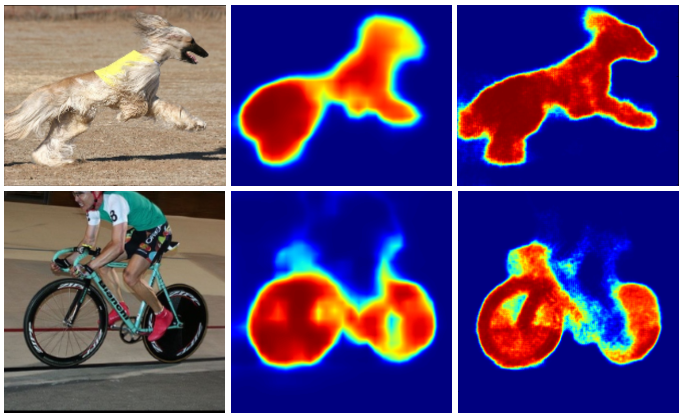
\includegraphics[width=.49\linewidth, trim=0 230px 0 0, clip]{../figures/fcnupsample.png}}
  \subfigure{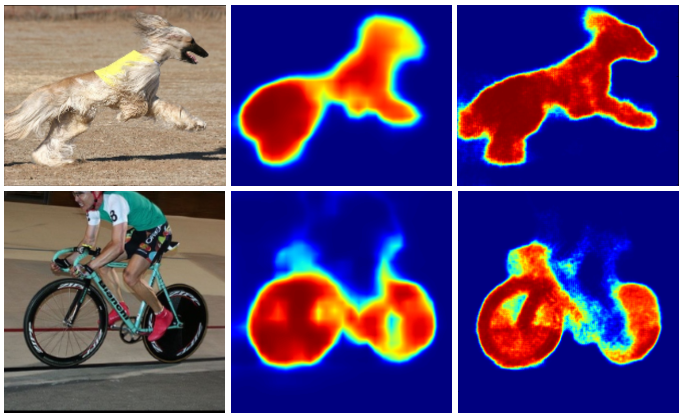
\includegraphics[width=.49\linewidth, trim=0 33px 0 200px, clip]{../figures/fcnupsample.png}}
  \caption{Comparison of upsampling a base image using FCN~\cite{fully-CNNs-for-semantic-segmentation} and the VGG-16-based DeconvNet~\cite{noh2015learning, simonyan2014very} architectures.}\label{fig:fcn-vs-deconvnet}
\end{figure}

This first convolutional network spawned a vicious flurry of convolutional architectures, which followed in their footsteps. The Fully Connected Neural Network (FCN) adapted the architecture used by LeCunn et al.~\cite{Lenet1998} for segmentation applications. Previously, convolutions would reduce input image feature vectors into non-spatial classification outputs. However, this paper `convolutionalized' the pipeline to provide a heatmap of segmented objects within the image~\cite{fully-CNNs-for-semantic-segmentation}. The heatmap would describe in a 2D feature the location of each class.

Trivial upsampling through de-convolutional layers allows the heatmap to translate back to the original size. This process would produce a largely inaccurate segmentation with much room for improvement. Therefore, similarly to learning the downsampling, the model learnt to upsample low-level heatmap representations~\cite{noh2015learning}. This way, the deconvolutional network also became ``a key component for precise object segmentation,'' which improved the base upsampling provided by the FCN. This conclusion is shown in Figure~\ref{fig:fcn-vs-deconvnet}.

The strategy of downsampling and upsampling for image segmentation is a common theme amongst many segmentation architectures.

\subsection{UNet}

\begin{figure}[H]
  \centering
  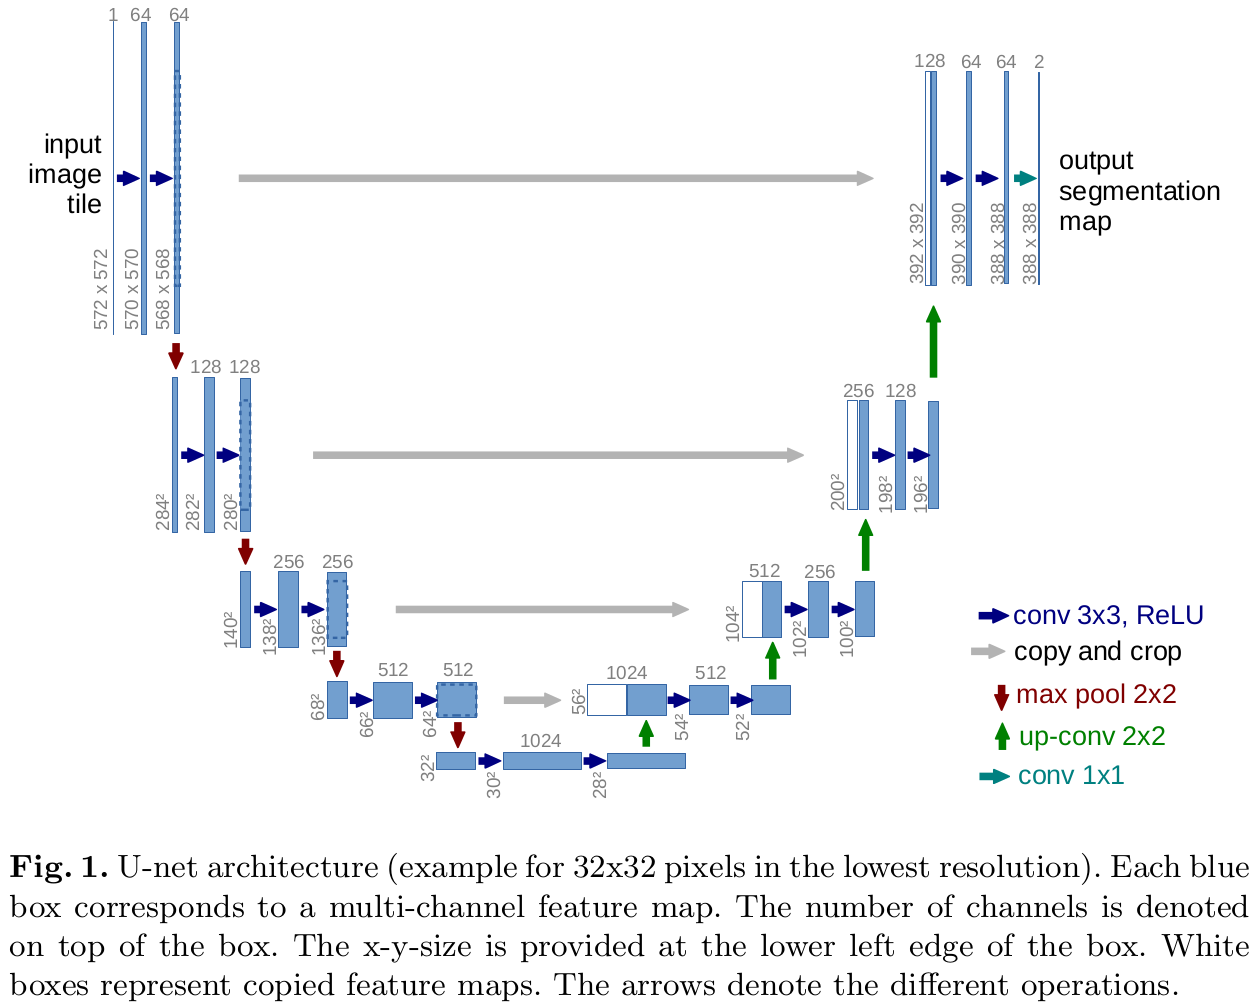
\includegraphics[width=.9\linewidth, trim=0 200px 0 0, clip]{../figures/u-net.png}
  \caption{The U-Net architecture, with contractive side on the left, and expansive side on the right. The feature map follows the arrows and multiplies the number of feature maps twice at each contraction, and halves at each expansion~\cite{U-Net}.}\label{fig:unet}
\end{figure}


Simultaneously, a unique architecture was under development. This architecture mirrored the hourglass structure of contracting and upsampling sections of the FCN, only this time, the illustration of its architecture led to its name, the UNet~\cite{U-Net}.

The UNet similarly consists of a contractive and expansive side, with the added feature of so-called `skip-connections'. As shown in Figure~\ref{fig:unet}, at each stage of the contracting/expansive side, these copy operations help localise high-resolution features from the contracting path~\cite{U-Net}. The network yielded great results for a few training images and more precise segmentations.

The U-Net was now very close to being a staple choice in biomedical data for anatomy segmentation. A limitation of its current implementation is that slices along the third dimension would most certainly contain contextual information that would influence the decision of the current design. Therefore, an identical network topology with extended 3D convolutions was proposed by \c{C}i{\c{c}}ek et al.~\cite{DBLP:journals/corr/CicekALBR16}.

\subsection{nnUNet}

Until now, architectures have operated on data pre-processed to a particular expected distribution and configured to deal with a specific problem. For instance, out-of-the-box configuration has stringent input size requirements, which require image resizing. Furthermore, 3D images commonly produce heterogeneous voxel spacing depending on the parameters chosen by the clinician or the machine from which they were produced~\cite{nnunet}. The number of moving parts often leaves a unidirectional dependency on the data depending on the architecture. 

Therefore, the nnUNet analyses the fingerprint of the dataset and the device to deliver a tailored experience and force a more codependent relationship; now, the architecture depends on the data and the data is pre-processed to conform to the network~\cite{nnunet}. Furthermore, hardware restrictions mean networks may be inaccessible to those with worse specifications or, at the other end of the spectrum, may underutilize powerful computation still available~\cite{nnunet}; the nnUNet analyses GPU constraints used to influence batch sizes and more~\cite{nnunet-git-paper}.

The automated method configuration is classified into three categories. A dataset fingerprint extracts training data distributions such as shape, spacing and intensity distributions. Rule-based parameters estimate the most common robust parameters for resampling and normalization. Finally, the Empirical Parameters learn parameters, such as ensemble selection, which is not derivable from the dataset fingerprint.

A review of segmentation methods in 2024 reviewed some further developments in segmentation models and found that the convolution-based U-Net architectures continued to outperform Attention-based or Mamba-based approaches six years after the initial publication of the self-configuring network~\cite{isensee2024nnunet}. Isensee et al. concluded that there was a significant mischaracterisation of proclaimed improvements in new strategies such as transformers. Claims of performance improvements over the nnUNet were reviewed through the control of validation datasets and removals of baseline tampering, which demonstrated the convolution-based performance on datasets with low statistical intra-method standard deviation~\cite{isensee2024nnunet}.

The continued performance dominance gives the nnUNet a good foundation for being used as a baseline model for all datasets.

\subsection{TotalSegmentator}

Total Segmentation is a tool with an nnUNet backbone pre-trained on 1204 CT examinations to provide plans to segment 104 anatomical structures. The anatomies selected included apparent structures such as skeletal structures, gastrointestinal organs and other major organs. The training data contained many CT images, with differences in slice thickness, resolution, and contrast phase~\cite{totalsegmentor-paper}. However, it is important to note that 60\% of the scans occurred in a contrast-enhanced environment, which plays a role in how obvious delineations are during scanning, a scanning detail that was omitted during the training data collection for this research project. Furthermore, only an estimated 10\% of the data collected from this model contained relevant studies for the abdomen and pelvic areas.

From the segmented organs that total segmentator provides, only the Bladder overlapped with the organs that were of interest in this study.

\subsection{UniverSeg}

\begin{figure}[H]
  \centering
  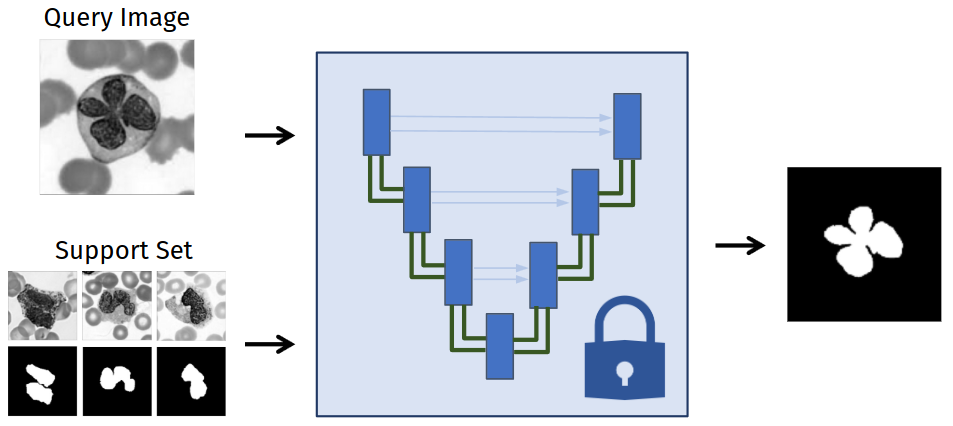
\includegraphics[width=.5\linewidth]{../figures/universeg.png}
  \caption{The UniverSeg architecture~\cite{universeg}. Diagram illustrates the freezing of model parameters while providing a support set of images which follows the query image through the segmentation pipeline.}\label{fig:universeg}
\end{figure}

Butoi et al. present UniverSeg, a model that breaks away from the traditional approach. Instead of training a model and freezing parameters during inference, this architecture uses a support set of images to provide a practical few-shot approach to inferring segmentations from input images. Figure~\ref {fig:universeg} shows an example of this efficient querying. This way, Butoi et al. attempt to provide segmentation on a target image based on examples of other samples with the same anatomy contoured in a selection of other images.

This model operates on 2D slices of images and directly avoids the finetuning argument for medical imaging. They argue that finetuning can be unhelpful due to the differences between medical domains, features, and data fingerprints. As such, UniverSeg avoids significant retaining for each subtask.

% Fully transferable, no retraining, few shot learning

% This is especially problematic in the medical domain where clinical researchers or other scientists are constantly defining new segmentation tasks driven by evolving populations, and scientific and clinical goals. To solve these problems they need to either train models from scratch or fine-tune existing models.

% Fine-tuning models trained on the natural image domain can be unhelpful in the medical domain [ 82 ], likely due to the differences in data sizes, features, and task specifications between domains, and importantly still requires substantial retraining. 

% Universeg avoids substatial retraining for each subtask

\subsection{SAM}

\begin{figure}[H]
  \centering
  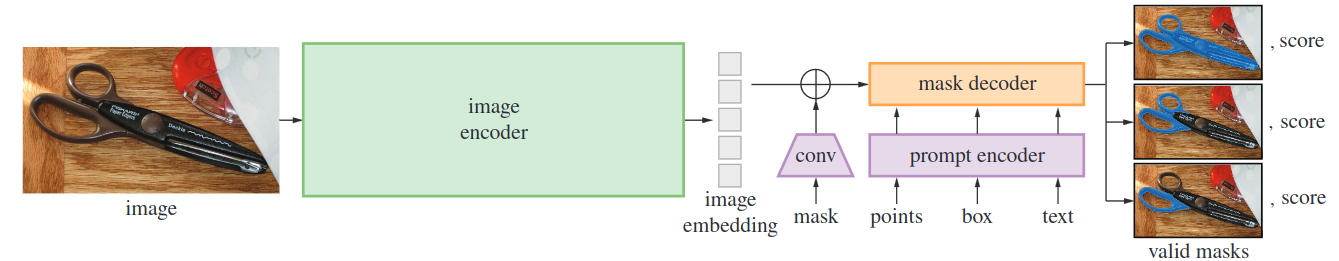
\includegraphics[width=1\linewidth]{../figures/SAM.png}
  \caption{The SAM model involves a transformer architecture that embeds points and bounding boxes into a promptable encoding, which is used in tandem with the image encoding to produce the most likely segmentation of the described area~\cite{SAM}.}\label{fig:sam}
\end{figure}

Up until recently, the segmentation methods have been convolution-based. However, advances in NLP with attention-based mechanisms prompted the adaption of transformers into the image domain~\cite{attention, ViT}. A vision transformer (ViT) views the image as a grid of tokens; in the original paper, Dosovitskiy et al. separate the image into a grid of patches and read in these cells of the grid as individual tokens. The tokens pass through the attention mechanism as with NLP and into a classification mechanism~\cite{ViT}. 

The SAM model implemented a modification of the transformer architecture~\cite{SAM} as seen in Figure~\ref{fig:sam}. However, the task was reformulated as a promotable segmentation problem to allow for zero-shot generalisation (the model can generalise to unseen examples with no re-training or fine-tuning).

\begin{figure}[H]
  \centering
  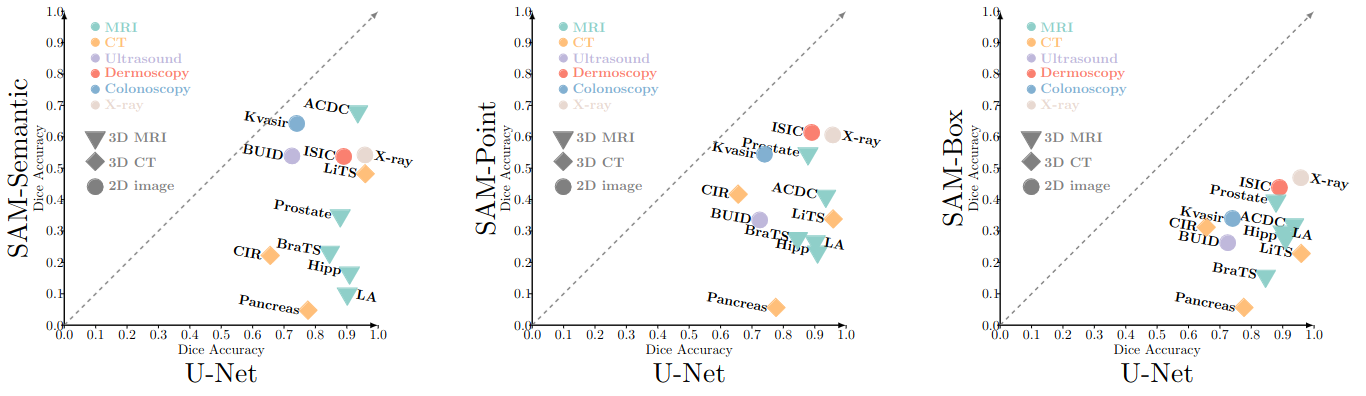
\includegraphics[width=1\linewidth]{../figures/sam-performance.png}
  \caption{Performance of a SAM (todo, was this finetuned?) model across a reference nnUNet baseline when applied to different datasets. The evaluation was considered for semantic, point and box prompts.~\cite{he2023computervision}.}\label{fig:sam-performance}
\end{figure}

SAM trains its network on a collection of natural images, not medical images such as CT and MRI scans. Extensive stress tests performed on SAM concluded that SAM's out-of-the-box promotable segmentation tool had good baseline performance on large visible objects~\cite{deng2023segment} but required exact prompt segmentation, making it inaccessible to automated contouring. Regarding the number of points required to make a sensible prediction, SAM quantitatively underperformed a nnUNet baseline, with qualitative evaluation showing fuzzy boundaries in medical contexts~\cite{hu2023sam}. Finally, Figure~\ref{fig:sam-performance} shows the performance of SAM against an nnUNet baseline across a set of datasets and imaging modalities~\cite{he2023computervision} which concludes that SAM never outperformed the nnUNet baseline when trained on the 11M natural images~\cite{SAM}. 

Thus, Ma et al. further reinforced the task to utilize a dataset of nearly 500k CT scan test examples to train a model for medical images, named MedSAM~\cite{Ma2024}. Ma et al. decided to keep close to its original despite medical images being 3-dimensional in CT and MRI scans because of ``enhanced flexibility and adaptability'' where slices along an axis substitute 3D scans~\cite{Ma2024}.

Thus, Ma et al. further reinforced the task to utilize a dataset of nearly 500k CT scan test examples to train a model for medical images, named MedSAM~\cite{Ma2024}. Ma et al. decided to keep close to its original despite medical images being 3-dimensional in CT and MRI scans because of ``enhanced flexibility and adaptability'' where slices along an axis substitute 3D scans~\cite{Ma2024}. This model demonstrates an improvement over SAM, nnUNet, and Deepmedic models when MedSAM bounding boxes extracted from the ground truth prompt the model~\cite{Ma2024}.

\clearpage

\section{Performance Evaluation for Segmentation Methods}\label{sect:performance-evaluation}

Calculating the difference between the provided labelled data would be one way to determine if a contour can be used in a clinical context. However, we have different ways to evaluate this measure in a delineation context.

If we were attempting to fit a model onto a line in 2D space, the performance of our model would be the total minimum distance between each point and the prediction. Our objective would be to drive the model's distance metric as close to 0 without overfitting. Here, the points act as a 'ground truth', alternatively referred to as the gold standard, which represents the actual measured value.

The reasoning above extends to 3D and 2D in a segmentation context with variants to measure other quantities, like the minimum distance between prediction and truth or the extent of volume overlap between the two. These are examples of geometric measures, which Mackay et al. has found to be the most popular measure in segmentation tasks~\cite{review-metrics}.

\subsection{Classification Based}\label{sect:classification-based}

Assesses if voxels within and outside the auto-contour have been correctly labelled~\cite{review-metrics}. To begin, we define 'positive' to mean that the voxel selected indeed needs radiotherapy treatment and 'negative' to mean that the voxel classifies as healthy.

A standard measure of classification is accuracy. It measures the total number of correct predictions vs. the total predictions it made. However, more than this measure is needed to fully capture a model's bias because it does not tell the whole story with class-imbalanced data when there is no even number between positive and negative labels.

\begin{equation*}
 \text{Accuracy} = \frac{TP + TN}{TP + TN + FP + FN}
\end{equation*}

Better measures are Precision and Recall scores. The Precision (also known as the Positive Predictive Value~\cite{evaluation-metrics}) measures the proportion of successfully correct predictions. The Recall (also known as True Positive Rate~\cite{evaluation-metrics}), on the other hand, ``measures the portion of positive voxels in the ground truth that is also identified as positive by the segmentation being evaluated''.

\begin{equation*}
 \text{Precision} = \frac{TP}{TP+FP}, \quad \text{Recall} = \frac{TP}{TP+FN}
\end{equation*}

\subsection{Spatial Overlap Based}\label{sect:spatial-overlap-based}

Similarly to classification-based metrics in Section~\ref{sect:classification-based}, an overlap-based metric measures the extent of overlap between an auto-contour and a reference structure~\cite{review-metrics}.

The scores above combined into a more general score $F_\beta$ to give

\begin{equation*}
 \text{F}_\beta = (1+\beta^2)\cdot \frac{\text{Precision} \cdot \text{Recall}}{\beta^2 \cdot \text{Precision}+\text{Recall}}
\end{equation*}

A specific case of this equation with $\beta=1$ is mathematically equivalent to the DICE Similarity Coefficient. A review found that DICE is the most popular evaluation metric amongst 2021 studies~\cite{review-metrics,evaluation-metrics, Sherer2021-le}.

% \begin{align*}
%   F_1 = \text{DICE} & = \frac{2 \cdot \text{Precision} \cdot \text{Recall}} {\text{Precision} + \text{Recall}} & \\ 
%   % & = \frac{2 \cdot \frac{TP}{TP + FP} \cdot \frac{TP}{TP + FN}}{\frac{TP}{TP + FP} + \frac{TP}{TP + FN}} \\
%   % & = \frac{2 \cdot TP \cdot TP}{TP(TP+FN)+TP(TP+FP)} \\ 
%   & = \frac{2 \cdot TP}{2TP + FP + FN} \quad = \quad \frac{2|S_g^1\cap S_p^1|}{|S_g^1|+|S_p^1|} , \text{where} \begin{cases}
%     S_g^1 & \text{ground truth} \\
%     S_p^1 & \text{segmentation}
%   \end{cases}
% \end{align*}

\begin{equation*}
 F_1 = \text{DICE} = \frac{2 \cdot \text{Precision} \cdot \text{Recall}} {\text{Precision} + \text{Recall}} = \frac{2 \cdot TP}{2TP + FP + FN} \quad = \quad \frac{2|S_g\cap S_p|}{|S_g|+|S_p|}
\end{equation*}

Where $S_g$ is the ground truth segmentation and $S_p$ is the predicted segmentation. From this relationship, the DICE score has found popularity in image segmentation for similar reasons that the $F_1$ score has found its popularity in classical machine learning; it can provide a fair result for imbalanced datasets. This mentality is applicable in our scenario because a tumour will make up very little of the total volume of the domain space. This argument extends to a Volumetric DSC by considering the above in all three dimensions~\cite{APL}.

Another popular related evaluation method is the Jaccard Index, which measures the intersection over the union of two sets:

\begin{equation*}
 \text{JAC} = \frac{TP}{TP+FP+FN} = \frac{|S_g\cap S_p|}{|S_g \cup S_p|} \iff \frac{DICE}{2 - DICE}
\end{equation*}

Since the numerator for the Jaccard Index is smaller than the DICE (since we avoid the issue of counting the intersecting sections twice), the JAC is always larger than the DICE score.

\subsection{Surface Based}\label{sect:surface-based}

Also commonly known as Boundary-Distance-Based Methods~\cite{boundary-overlap-metrics} compares the distance between two structure
surfaces. These can be maximum, average or distance at a set percentile of ordered distances~\cite{evaluation-metrics}.

A typical example is the Haussdorf Distance. Here, a directed distance metric is the maximum distance from a point in the first set to the nearest point in the other between two individual voxels~\cite{boundary-overlap-metrics}. Therefore, the better the HD metric, the smaller the value it returns. Here, the distance is typically Euclidian distance.

\begin{equation*}
 \text{HD}(A,B) = \max(h(A,B), h(B,A)), \quad \text{ and directed h}(A,B)=\max_{a\in A}\min_{b \in B} ||a-b||
\end{equation*}

The HD is generally sensitive to outliers; therefore, direct HD application gives uninspiring results because noise and outliers are common in medical segmentations~\cite{boundary-overlap-metrics}. Therefore, we can calculate the average directed Haussdorf Distance.

\subsection{Volume Based}

Volume-based metrics consider only the volume of the segmentation~\cite{evaluation-of-metrics-in-prostate,review-metrics, boundary-overlap-metrics}. However, its poor spatial descriptions make it more commonly used jointly with other metrics.

\begin{equation*}
 \text{Relative Volume Difference (RVD)} = \bigg| \frac{|S_g|-|S_p|}{|S_g|}\bigg|
\end{equation*}

\subsection{Evaluation}\label{sect:evaluation-of-evaluation-methods}

All these methods can be advantageous in some places rather than others. To decide which segmentation is best, we can list some challenging scenarios.

\begin{figure}[H]
  \centering
  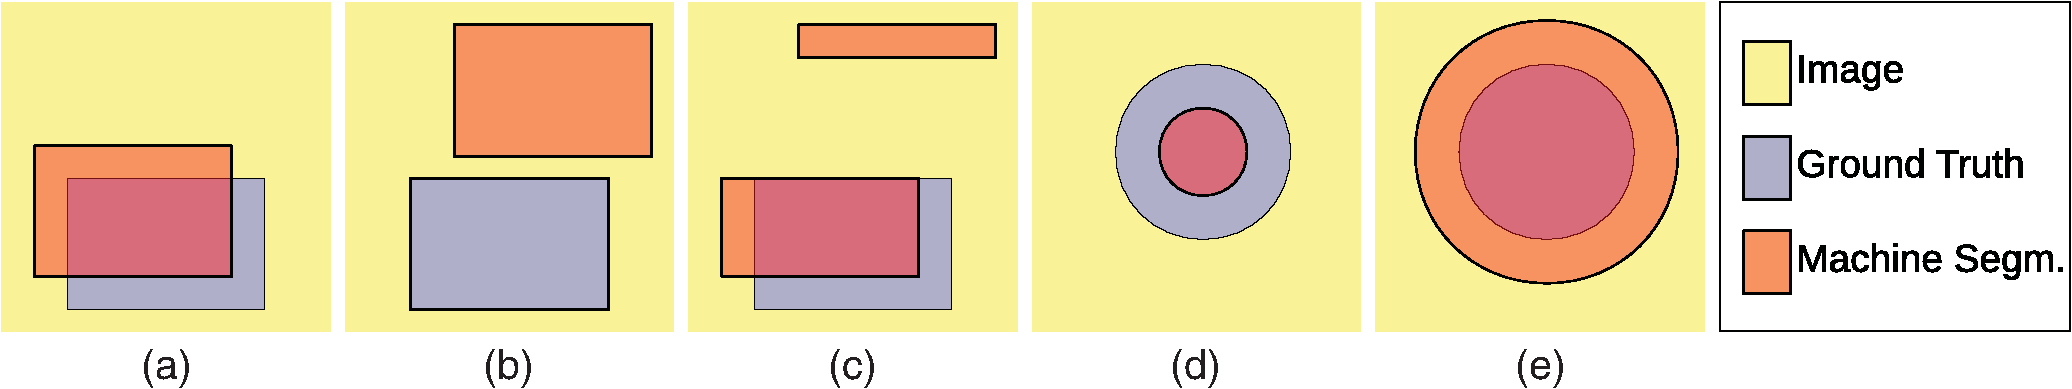
\includegraphics[width=\linewidth]{../figures/segmentation-cases-1.png}
  \caption{Figure from~\cite{boundary-overlap-metrics} illustrating cases of segmentation to aid with explanation of set-backs of certain evaluation metrics}
 \label{fig:segmentation-cases-1}
\end{figure}

\begin{itemize}
  \item Classification Based (Section~\ref{sect:classification-based}) and Spatial Overlap Based (Section~\ref{sect:spatial-overlap-based}) are similar; they are concerned with the number of correctly classified or misclassified voxels without taking into account their spatial distribution. Here, Figure~\ref{fig:segmentation-cases-1}(a) and Figure~\ref{fig:segmentation-cases-1}(c) would achieve similar results despite Figure~\ref{fig:segmentation-cases-1}(a) being locally bound to a better area.
  \item With Haussdorf Distance (Section~\ref{sect:surface-based}) output segmentations generated by Figure~\ref{fig:segmentation-cases-1}(d) and Figure~\ref{fig:segmentation-cases-1}(e) will result in the same score, which is not favourable in a radiotherapy planning environment where an organ-at-risk is involved.
  \item Figure~\ref{fig:segmentation-cases-1}(b) would score flawlessly when using volumetric score estimation. However, it does not consider spatial placement, making this measurement poor when used individually.
\end{itemize}

\subsection{Estimated Editing Based}\label{sect:surface-dice}

Selecting a measurement that can reflect a clinician's acceptability score is difficult. A study found a lack of correlation between a geometric index and expert evaluation, with the JAC score having a 13\% False Positive Rate. The study's conclusion summarised that scores such as JSC and volumetric DSC ``provide limited clinical context and correlation with clinical or dosimetric quality''~\cite{Sherer2021-le}.

% Because of the clinical context of evaluating the segmentation by a machine, it may sometimes be helpful to define a performance metric as the ``fraction of the surface that needs to be redrawn''~\cite{Nikolov2021-xe} since models at this point require manual review to avoid automation bias (Section~\ref{sect:using-the-tool}). This method is helpful for larger structures as it doesn't assign much weight to the large trivial internal volume, which accounts for a much more significant proportion of the score.

\subsubsection{Surface DSC}\label{sect:surface-DSC}

The study at~\cite{Sherer2021-le} helped drive an initiative to combine aspects of surface Based evaluation (Section~\ref{sect:surface-based}) and Spatial Overlap Based evaluation (Section~\ref{sect:spatial-overlap-based}) into a Surface DICE which assesses the specified tolerance instead of the overlap of the two volumes.

\begin{figure}
  \centering
  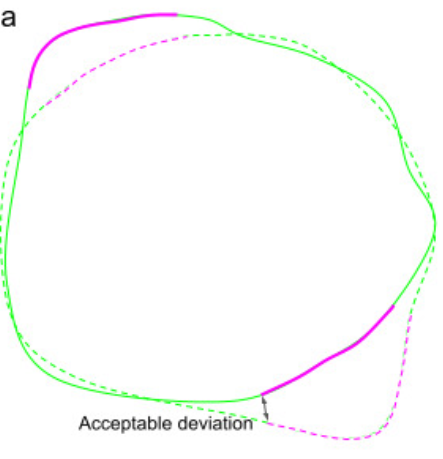
\includegraphics[width=0.3\linewidth]{../figures/Surface-dice.png}
  \caption{Taken from~\cite{Nikolov2021-xe}. Illustrates the computation of the surface DICE, where the continuous line is the predicted surface, and the dashed line is the ground truth. The black arrows show the maximum deviation tolerated without penalty; therefore, in pink are the unacceptable deviations and green otherwise.}\label{fig:surface-dice}
\end{figure}

We can formulate the Surface DSC score in a mathematical definition~\cite{Sherer2021-le} with its corresponding illustration in Figure~\ref{fig:surface-dice}.

\begin{equation*}
 \text{Surface DSC} = \frac{|S_p \cap B_{g,\tau}| + |S_g \cap B_{p,\tau}|}{|S_p| + |S_g|}
\end{equation*}

This definition measures the agreement between just the surfaces of two structures above a clinically determined tolerance parameter, $\tau$. Here, $B_{p,\tau}$ represents the boundary region of the predicted surface within a maximum margin of deviation $\tau$ and similarly for $B_{g,\tau}$ for the ground truth.

\subsubsection{Added Path Length}

Similarly, the APL score predicts ``the path length of a contour that has to be added''~\cite{APL}. APL achieved similarly by considering the number of added voxels required between the prediction and the gold standard with no regard to tolerance as a pose to Surface DSC (Section~\ref{sect:surface-DSC})

% \begin{warning}
%  For future reference, \textit{\href{https://stackoverflow.com/questions/73286639/how-to-calculate-added-path-length-apl-image-segmentation-metric}{stack overflow discussion}}

%  Implementation of surface DSC and APL: \textit{\href{https://github.com/pyplati/platipy/blob/master/platipy/imaging/label/comparison.py}{source code}}
% \end{warning}

\subsection{Summary}

This is why we settle at the Surface DSC (Section~\ref{sect:surface-dice}), which prioritizes deviation along the boundary to a certain degree while measuring the fraction of the surface that needs to be redrawn, thus favouring a more conservative prediction of Figure~\ref{fig:segmentation-cases-1}(d) instead of (e).

For this project, we shall select an evaluation measurement more biased towards conservative boundary estimates not to touch the organs at risk. The clinician's review pipeline, in part, influenced this choice; it would be easier to correct Figure~\ref{fig:segmentation-cases-1}(d) instead of Figure~\ref{fig:segmentation-cases-1}(e) because correcting the latter would likely take a considerable amount of time as it would require redrawing almost all of the boundary, whereas the former could be corrected much faster~\cite{Nikolov2021-xe}.



%%%%%%%%%%%%%%%%%%%%%%%%%%%%%%%%%%%%
\chapter{Methodology}\label{sect:methodology}

A simple nnUNet model can be trained from scratch to provide an accurate segmentation for anatomy and radiotherapy target volumes. This nnUNet model has been shown to provide more robust results in external stress tests than other comparable architectures on a set of different datasets~\cite{isensee2024nnunet}. Also, in many biomedical applications, ``only very few images are required to train a network that generalises reasonably well''~\cite{DBLP:journals/corr/CicekALBR16}.

However, improvements over the baseline could hypothetically allow the segmentation of delineated areas more accurately.

\section{Transfer Learning}

A strategy for improving the accuracy of a model is Transfer Learning.

Transfer Learning involves transferring a model's knowledge from a domain that has trained on more volumes of training data in another domain and is used as a starting point in the target domain. Transfer is a source of success because, in the early layers of a model, it typically learns very low-level features. At 
this scale, the objective of the original domain does not matter; regardless of the initialisation, a model working on a similar problem will inevitably learn similar low-level features. 

Arguably, the universality of the parameters learnt in a model with prosperous access to data will have richer and better patterns that another with less data did not have enough information to learn~\cite{deep-learning-book, survey-on-transfer-learning}.

Transfer Learning has the potential to improve initial performance using only the transferred knowledge before any further learning begins, improve the time it takes to thoroughly learn the target task given the transferred knowledge, and improve the final performance all when compared to initial benchmarks without transfer~\cite{torrey-handbook}. Medical contexts have already applied Transfer Learning, which reportedly improved weight initialisation for 332 abdominal liver CT scans and resulted in faster convergence, providing a more robust representation~\cite{liver-lesion-via-transfer-learning}.

Transfer Learning has been seen to prevent overfitting in domains where data volume is low and where generality without overfitting is hard to come by. The prevention is because the model has already learnt features likely to be helpful in the second task~\cite{geeks-transfer-learning}. 

However, generalisation is not a guarantee, as overfitting is still possible if the model is fine-tuned too much on the second task, as it may `learn task-specific features that do not generalise well to new data'~\cite{geeks-transfer-learning}. In our case, our target dataset is small but similar to the base network dataset. We may overfit because fine-tuning the pre-trained network with the target dataset may not generalise to the global population. If, instead, we attempt to transfer a task with a different base network dataset, then using high-level features of the pre-trained model will not be useful~\cite{geeks-transfer-learning}.

\section{Base-line nnUNet...}

%%%%%%%%%%%%%%%%%%%%%%%%%%%%%%%%%%%%
\chapter{Results}\label{sect:results}

...

%%%%%%%%%%%%%%%%%%%%%%%%%%%%%%%%%%%%
\chapter{Discussion}\label{sect:discussion}

Here, discuss results from all 4 of the methods tested.

% total segmentator had 500 females to 700 males which may explain the struggle to locate the uterus and vagina.


%%%%%%%%%%%%%%%%%%%%%%%%%%%%%%%%%%%%
\chapter{Conclusion}

Transfer works!

% because of the way the CTV is drawn based on the progression of the tumor and how far along the patient is, this influences the contour drawen. Perhaps, the metrics suggest that a model with only one modality is not enough to make a decision which sparks the idea of a model which is capable of multi-modal analysis.

%%%%%%%%%%%%%%%%%%%%%%%%%%%%%%%%%%%%
\chapter{Ethics}

The lack of effort to protect the identities and confidentiality of patients during research projects may result in ``stigma, embarrassment, and discrimination''~\cite{health-privacy} if the data is misused.
This project involves the intimate and personal information of many female patients whose privacy must be protected before research occurs.

\section{Patient disclosures}

Researchers may collaborate with third parties, such as Imperial College London, by providing anonymised data that third parties cannot reverse-engineer to identify the patient. The collaborating hospital, The Royal Marsden Hospital, does not require ``explicit consent'' for sharing collected clinical data with outside entities as long as the patient is made aware of the ways their ``de-identified/anonymised'' data may be used.~\cite{royal-marsden-privacy-note}. Imperial College's Medical Imaging team also arranges formalities, such as acting as "ethical data stewards"~\cite{Larson2020-ib}. 

The MIRA team acts as responsible data stewards by storing anonymised data within a folder on the college network. They received all provided data in the \texttt{NIfTI} file format, which discloses no personally identifiable information, as defined by the GOV website~\cite{gov-gdpr}. Specific access rights limit data availability in this folder, ensuring security measures. Moreover, taking the data outside this folder reduces individual patient risk through the exchange of de-identified data.

Without such disclosure, anonymisation, and a security guarnatee of the data, patients may be reluctant to provide candid and complete disclosures of their sensitive information, even to physicians, which may prevent a complete diagnosis if their data is not maintained anonymously.

\section{Using the tool}\label{sect:using-the-tool}

The applications of this tool bode well in the healthcare ecosystem as the community slowly accepts the involvement of AI-powered medical tools. Radiology is one application that has been most welcoming of the new technological advances as there is potential for substantial aid by reducing manual labour, increasing precision and freeing up the primary care physician's time~\cite{Amisha2019-ki}.

However, it is too early to take the results of the medical tool as gospel. For current cervical radiotherapy delineation tools, only 90\% of the output is acceptable for clinical use~\cite{LIU2020172}. Therefore, The remainder can potentially cause more harm than good if not checked properly. For example, the overlap of a PTV with an organ-at-risk may invoke a cascade of adverse effects for the patient. The remaining 10\% of outputs may score incorrectly because the model uses a single modality, but physicians may base their final judgement on a multivariate analysis. Therefore, clinicians should use the tool as a second opinion rather than a primary source of information. Otherwise, an ethical dilemma of establishing the responsible party for incorrect decisions made by DL tools should also be determined~\cite{Chen2021-dg}.

Clinicians can fall into the trap of automation bias as AI becomes more commonplace in clinical environments~\cite{STRAW2020101965}. However, many models of this age codify the existing bias in common cases, which often will fail those patients who do not fit the majority's expectations. 

Therefore, before integrating tools into workflows, a committee must establish the degree of supervision required from physicians if this tool is to be used in practice. Currently, oncologists will be required to reverse-engineer the `black box' results to verify why a decision has been made. 

%%%%%%%%%%%%%%%%%%%%%%%%%%%%%%%%%%%%

%% bibliography
\bibliography{../.latex-templates/references}

\end{document}